% R18: official Wiley USG class from supplied November 2026 template.
% Anonymous manuscript; use separate title pages for author information.
\documentclass[HARVARD,twocolumn]{USG}
\usepackage{mathtools}
\usepackage{etoolbox,lastpage}
\graphicspath{{images/}{figures/}}
\newcommand{\unit}{kg CO$_2$e/MWh}
\providecommand{\doi}[1]{\href{https://doi.org/#1}{doi:\allowbreak #1}}
\bibpunct{(}{)}{;}{a}{,}{,}
\hypersetup{hidelinks,pdfauthor={},pdftitle={The Opportunity Cost of Carbon Calculation Errors in Green Capital Budgeting}}
\articletype{ORIGINAL ARTICLE}
\journal{Business Strategy and the Environment}
\startpage{1}
\copyyear{2026}
\articledoi{}
\historydates{}
% The official class prints publisher-assigned bibliographic data by default.
% For a submission draft, replace only the first-page footer, not the class file.
\makeatletter
% Subscription-route draft: suppress the template's unconditional OA icon.
\patchcmd{\@@articletype}{\raisebox{-2\@p@t}{\includegraphics[width=0.70in]{images/openaccess}}}{}{\typeout{R17: removed default OA badge}}{\PackageError{R17}{OA badge suppression failed}{Inspect template version.}}
% Correct the supplied class's draft footer and avoid a publisher DOI/volume.
\newcommand{\rseventeenfooter}{\vbox{\hsize\textwidth\hrule height .5\p@\vskip3\p@\hbox to \textwidth{\fontsize{7}{9}\selectfont\textit{Business Strategy and the Environment} --- Manuscript for peer review\hfill\thepage\ of \pageref*{LastPage}}}}
\def\oddfoot@titlepage@box{\rseventeenfooter}
\def\oddfoot@titlepage@info{\rseventeenfooter}
\def\evenfoot@titlepage@info{\rseventeenfooter}
\def\oddhead@titlepage@info{}
\def\evenhead@titlepage@info{}
\def\oddhead@headings@info{\rseventeenfooter}
\def\evenhead@headings@info{\rseventeenfooter}
\patchcmd{\@maketitle}{\foot@measure\enlargethispage{-\foot@raise}}{}{\typeout{R17: removed obsolete first-page footer lift}}{\PackageError{R17}{Footer patch failed}{Inspect template version.}}
\makeatother
\begin{document}
\title{The Opportunity Cost of Carbon Calculation Errors in Green Capital Budgeting}
\authormark{Carbon errors and green budgeting}
\titlemark{Carbon errors and green budgeting}
\keywords{carbon accounting | environmental strategy | green capital budgeting | sustainability assurance | capital allocation | opportunity cost}
\abstract[ABSTRACT]{Carbon calculation errors can increase portfolio net present value (NPV) while displacing investments that meet an environmental mandate. We derive an exact decomposition of qualified NPV shortfall into exclusion and displacement losses. For indivisible projects with positive additive costs, additive values, one budget and optional unspent capital, displacement occurs precisely when ineligible spending exceeds the capital remaining after reserving the least expensive optimal portfolio of projects passing both calculations. Across 48 constructed energy projects in eight portfolios, two intensity-understatement errors changed 129 funding decisions; 55 retained all reference investments. At three matched error scales, overstating intensity produced a larger mean qualified NPV shortfall under every joint reassignment of financial profiles, averaging equally over portfolios, budgets and ceilings. This ordering could reverse at the 45\% budget. The findings provide an exact decision criterion for carbon-accounting assurance before capital commitment.}

\maketitle
\section{Introduction}
Carbon calculation errors can undermine the execution of an environmental investment mandate even when the selected portfolio generates a positive financial return. This study derives an exact capital-displacement condition and tests it in eight constructed energy-project portfolios. In one of these portfolios, a lender funds a USD 40 million energy project because of a single choice in the carbon calculation. The lender sets a ceiling on emissions per unit of electricity delivered to the grid. The project exceeds that ceiling. Dividing the same emissions by all the electricity generated, including electricity that never reaches the grid, makes it appear to qualify. With USD 87.75 million to invest, the lender then drops two qualifying projects whose discounted future cash flows exceed their initial costs by USD 4.40 million in total. That is the net present value (NPV) forgone. With USD 117 million, it can fund the same USD 40 million project and keep both alternatives. What determines how much qualifying investment an error displaces?

Two public records illustrate why estimating that cost requires evidence about both the calculation and the financing decision. At Chile's Copiulemu landfill gas project, a verifier traced an error in the December 2006 methane calculation to a spreadsheet summing column O in place of column N \citep[p.~11]{sgs}. At Vasilikos Unit~6 in Cyprus, the European Investment Bank estimated emissions of about 380 grams of carbon dioxide per kilowatt-hour on natural gas. The estimate met the ceiling of 550 that still applied to projects already under appraisal. It exceeded the new ceiling of 250 \citep{eibscore,eibmid}. The bank signed a loan of EUR~76 million on 17 December 2020 \citep{eibloan}. The Chilean record identifies a formula error and the Cypriot record identifies a funded project. To measure financial displacement one would also need to know which other projects competed for the money.

Recent research in environmental management treats carbon accounting as a mechanism for translating organizational commitments into routines and decisions. \citet{ruan2026}, drawing on qualitative responses from 44 industry experts, describe how governance arrangements, capabilities and operational infrastructures embed carbon accounting in organizations. A mixed-method study by \citet{wu2026} synthesizes carbon accounting barriers, enabling conditions and strategies from 53 studies and industry-expert responses. These findings identify the organizational need to connect emissions information with decision processes. For a capital allocation rule, a concrete aspect of that connection is whether the implemented calculation produces the eligibility decision intended by the approved rule.

Clean energy finance brings measurement and capital allocation into the same decision. Target~7.a of Sustainable Development Goal~7 calls for investment in clean energy technology and infrastructure \citep{un}. A lender pursuing that aim can specify exactly which emissions to count and still face a financing problem if the calculation admits the wrong project. The amount lent is visible in its accounts. The value of the qualifying projects it passed over must be reconstructed from the alternatives it faced.

We traced the calculation with a research engine developed to document key performance indicators (KPIs), the measures organizations use to track performance. Literate Programming for Automated KPI Extraction (LEAP) adapts the practice of presenting code alongside an explanation of what it does \citep{knuth,zenodo,leap}. Here it identifies the written emissions formula and the code that implements it. We compare the projects funded under the specified formula with those funded under each altered calculation. We derive the spending threshold at which financing a project admitted in error displaces qualifying value, then test how the loss varies with the budget and emissions ceiling. We also ask how many project eligibility checks would settle the funding decision if the formula in use were uncertain.

\section{From carbon measurement to investment choice}
Climate finance research links funding mechanisms to energy transition and climate resilience. In their hybrid review, \citet{joshipura2025} identify financing for the transition, eco-innovation, funding sources and enabling conditions as connected research themes. \citet{raimondi2026} synthesize approaches to integrating climate considerations into bank credit-risk assessment using academic and practitioner literature. These perspectives motivate the decision setting here: a financier has adopted a carbon-based investment mandate, and its practical implementation determines which projects can compete for capital.

Two analysts can start with the same companies and assign them different environmental scores. In comparing environmental, social and governance ratings, \citet{berg} traced disagreement to differences in what providers measure, how they measure it and how they weight the results. That disagreement can narrow the investment choice when a mandate requires several providers to agree \citep{lohmann}. \citet{tian2026} develops an accountability framework tracing ESG-rating divergence through the measurement process across jurisdictions. Distinct measurement choices can legitimately express different objectives. An implementation discrepancy exists when the executable calculation departs from the approved formula. Whether it changes eligibility depends on the calculated intensity and the specified ceiling. Carbon measurement poses a more specific question. Using two emissions datasets, \citet{anquetin} examined how counting emissions from suppliers and other activities along a company's value chain affects the construction of green equity portfolios. In each case, the measurement choice helps determine which assets an investor can hold or how much to invest in them.

For a lender financing whole projects, eligibility is only the first decision. A second project can qualify and still compete for the money needed to fund the first. This is the classic problem of capital rationing, in which the investor must allocate a fixed sum among competing investments \citep{lorie}. For building retrofits, \citet{he} evaluated which buildings and improvements to finance together, considering both financial returns and energy or emissions benefits. Another approach gives financial, environmental and social value explicit weights in the investment decision \citep{schoenmaker}. Our lender uses an emissions ceiling to determine eligibility and NPV to choose among affordable combinations. We call the combined NPV of funded projects that meet the ceiling under the specified formula their \emph{qualified NPV}. A project that fails the ceiling may generate a positive return while using capital needed by a qualifying alternative.

Sustainability assurance also has a documented relationship with environmental performance. Using panel regressions on 6,140 firm-year observations across 39 countries, \citet{ibrahim2026} associate higher sustainability audit quality with lower reported carbon-emission intensity. The present analysis addresses a decision-level mechanism within assurance: how correcting an erroneous eligibility calculation changes the attainable value under an already specified investment mandate.

Before attributing any loss to an error, an analyst needs to know what the carbon score was supposed to measure. Green bond research illustrates why the available evidence matters. \citet{nicolici} examined what issuers disclose about environmental monitoring, while \citet{loiola} distinguished bonds aligned with a financing framework from those formally certified under it. To check an individual calculation, the analyst also needs a rule precise enough to yield an expected value. An explicit rule and its inputs allow the analyst to test the calculation directly. In one LEAP example, the written rule defined gross margin as the share of revenue left after deducting costs. Revenue of 100 and cost of 60 therefore gave a margin of 40\%. The program returned 166.67\% on those inputs \citep{review}. In the present study, the corresponding comparison is between two emissions scores for the same project.

Does the analyst have to check every project before the lender can settle on a portfolio? \citet{schloter} studied which uncertain item values must be verified to identify an optimal selection. \citet{dughmi} studied which items to check for availability to obtain a near-optimal expected return. In our case the lender knows the cash flows and costs. Each check establishes whether one project meets the emissions ceiling. The lender can stop once it knows that the same projects will be funded however the outstanding checks turn out.

Knowing which projects will receive funding still leaves the central financial question open. When a calculation error changes eligibility, how much qualifying value does the investment committee forgo? Related work identifies the boundaries at which investment choices change. \citet{hien} examined how a margin for uncertainty alters the allocations allowed by a risk budget. \citet{pisinger} established exact tolerance intervals for individual profit or weight perturbations and used the least-weight optimum to maximize residual capacity. Here project values, costs and the emissions rule are fixed. The implemented calculation changes which projects are eligible. We use the residual-capacity principle to separate loss from excluded qualifying projects and loss from capital spent on falsely admitted projects, and to characterize when the latter loss begins. This connects a familiar optimization mechanism to a specific environmental investment decision.

\section{Materials and methods}
The lender makes two decisions in sequence. It screens each project against a ceiling on operating emissions per unit of electricity, then funds the qualifying combination with the highest NPV it can afford. The specified calculation and ceiling define the reference rule. We compare the reference decision with the decisions under three altered calculations, keeping the projects, cash flows and budgets fixed. This lets us value two ways the lender can lose a qualifying investment. The error can exclude the project outright, or it can admit another project that uses the capital needed to fund it. We also examine how many eligibility checks would settle the funding decision if the correct calculation were uncertain.

\subsection{Project inputs and carbon eligibility}
The study comprises eight constructed portfolios of six indivisible energy projects each. For project $i$, gross generation $G_i$ is the electricity it produces, and net exports $Q_i$ are the electricity it delivers to the grid. Both are measured in megawatt-hours, with $G_i>Q_i>0$. Scope~1 emissions $S_{1i}$ come directly from the project's operations. Scope~2 emissions $S_{2i}$ arise from producing the energy that the project purchases. Both quantities are measured in kilograms of carbon dioxide equivalent, following the Greenhouse Gas Protocol's scope terminology \citep{ghg}. The reference intensity $E_i=(S_{1i}+S_{2i})/Q_i$ therefore measures operating emissions per megawatt-hour exported. It excludes lifecycle and avoided emissions. A project qualifies when its calculated intensity is at or below the ceiling $\tau$.

The 48 project records include intensities near each study ceiling. Starting with six base intensities of 330, 378, 392, 407, 429 and 465~\unit, we adjusted them by portfolio and project position to place projects on either side of the three ceilings of 380, 400 and 420~\unit. Within each portfolio, capital cost and reference intensity both increase with project position. A higher-intensity project admitted by an altered calculation can therefore compete for a substantial share of the budget. Supplement~S1 gives the generator equations, project identifiers and raw inputs.

Four programs receive the same project inputs and declare the same formula. The reference program returns $E_i$. Using gross generation as the denominator gives $(S_{1i}+S_{2i})/G_i$ and lowers intensity because gross generation exceeds net exports by 7\% to 17\%. Omitting Scope~2 gives $S_{1i}/Q_i$ and lowers intensity because Scope~2 accounts for 9\% to 19\% of total emissions. Both percentages vary with the same combination of portfolio and project indices. The third alteration understates net exports, giving $(S_{1i}+S_{2i})/(0.85 Q_i)$ and raising intensity by a factor of $1/0.85$. In each primary comparison, all six projects in a portfolio use the same program.

\subsection{Capital budget and financial outcomes}
The financier ranks affordable project combinations by their combined NPV. Each project requires a positive initial outlay $K_i$ and generates five equal end-of-year net cash flows $C_i$. We assign no additional value after year five. At its project-specific annual discount rate $r_i$ between 7\% and 10\%, its NPV in modeled USD millions is $v_i=-K_i+\sum_{t=1}^{5} C_i/(1+r_i)^t$. The financier can spend $b$, set at 45\%, 60\% or 75\% of the capital needed for all six projects. Given the eligible set $A$, the best attainable NPV is
\begin{equation}
\begin{aligned}
 V(A,b)&=\max_{\substack{S\subseteq A\\ K(S)\le b}}v(S),\\
 K(S)&=\sum_{i\in S}K_i,\quad v(S)=\sum_{i\in S}v_i .
 \end{aligned}\label{eq:opt}
\end{equation}
where $K(S)$ and $v(S)$ are the total cost and NPV of a subset $S$. Write $S(A,b)$ for the chosen subset. The financier may leave part or all of the budget unspent, so the empty set is among the 64 possible subsets. Among equally valuable choices the program selects the least expensive. If costs also tie, a fixed subset ordering selects the first maximizer in that ordering. An independent calculation found a unique highest-value subset in every main and control decision.

We distinguish the financial value of the projects funded from the value they deliver under the reference rule. Let $T$ be the projects that qualify under that rule, $R$ the projects that qualify under the reported calculation, and $\widehat S=S(R,b)$ the funded set. Its total NPV includes all funded projects (the supplement calls this \emph{nominal NPV}). Its qualified NPV includes only the funded projects that pass the reference rule, $\widehat S\cap T$. Subtracting the qualified NPV delivered from the best NPV attainable under the stated rule gives the shortfall
\begin{equation}
 L=V(T,b)-v(\widehat S\cap T). \label{eq:loss}
\end{equation}
We also measure capital committed to ineligible projects as $K(I)$, where $I=\widehat S\setminus T$ contains the falsely admitted projects that received funding. These projects can still generate cash flows even though the mandate credits them with no qualified NPV.

\subsection{Value lost through exclusion and capital displacement}
Let $C=T\cap R$ contain the projects that pass both screens. Comparing $T$ with $C$ at the full budget measures the value lost through false exclusions. Keeping $C$ fixed and deducting the capital $K(I)$ spent on false admissions measures displacement. The two losses sum to the qualified NPV shortfall,
\begin{equation}
\begin{aligned}
L={}&\underbrace{V(T,b)-V(C,b)}_{\substack{\text{value removed by}\\\text{false exclusions}}}\\
&+\underbrace{V(C,b)-V(C,b-K(I))}_{\substack{\text{qualified value displaced}\\\text{by false admissions}}} .
\end{aligned}
\label{eq:decompose}
\end{equation}
To see why, hold the funded ineligible projects $I$ fixed. The qualified portion of $\widehat S$ must maximize NPV over $C$ at the residual budget $b-K(I)$. A more valuable affordable subset of $C$ could be funded alongside $I$ and would improve on the reported optimum. Substituting that residual-budget optimum into Equation~\eqref{eq:loss} gives Equation~\eqref{eq:decompose}.

Each component is nonnegative because removing projects or reducing the budget can only restrict the choice. If the altered screen only admits extra projects, displacement accounts for the entire loss. If it only excludes projects, exclusion accounts for the entire loss. For a mixed error we measure exclusions with all capital available before measuring displacement among the projects still eligible. This accounting assumes additive project costs and NPVs and allows capital to remain unspent.

The threshold for displacement is the capital left after reserving the least expensive optimal subset of $C$. Write $c^*(C,b)$ for its cost and $h=b-c^*(C,b)$ for the capital left. Then
\begin{equation}
\begin{gathered}
 V(C,b)-V(C,b-K(I))>0\\
 \Longleftrightarrow\quad K(I)>h .
 \end{gathered}\label{eq:slack}
\end{equation}
If $K(I)\leq h$, at least one common-eligible optimum still fits. If $K(I)>h$, every subset attaining the original value costs more than the residual budget. With finitely many subsets, the best attainable value must then fall. Choosing the least expensive of the tied portfolios therefore gives the threshold even when several portfolios have the same NPV.

\subsection{Source checks, controls and units of comparison}
Each of the 48 main projects had four small Python programs, one for each version of the formula. Together they provided 192 files in which to compare a documented rule with the calculation actually performed. LEAP read the explanatory notes in each file and returned the indicator's name, its declared formula and its location alongside the nearby code. A separate program compared the operations and their order in the declared and implemented formulas, using Python's structured representation of each expression. It also executed each file on the project's inputs and checked the output against the registered reference intensity. The financing model applied the ceiling to the computed value. A discrepancy in the source record did not itself trigger a new funding decision.

Two checks can flag the same document for different reasons. In a study of generated indicator documentation, the checker and the reviewers sometimes identified different problems in the same document \citep{checks}. Here one check asks whether the code performs the operations in the written formula. The other asks whether the result agrees with the expected value on the project's inputs. We recorded the answers separately and examined cases in which they differed. We also compared LEAP with a simpler program that read the first matching note in each file.

The eight portfolios are the units of analysis. Evaluating each at three ceilings and three budgets gives 72 conditions per implementation. Primary mean monetary outcomes give equal weight to all 72, including unchanged selections. Eligibility has a different denominator. Each project's status depends on the ceiling and is the same at every budget, giving $48\times3=144$ project--ceiling comparisons per implementation. Counts and means describe repeated decisions on these portfolios.

The 48 control projects reuse the financial inputs but place intensities away from the ceilings, using base values of 180, 220, 260, 560, 620 and 700~\unit. The original control program scanned its 192 source files and evaluated the four formulas directly. A separate replay executed each control file. An independent verifier reconstructed the project generator, checked eligibility with exact arithmetic and optimized all 288 main and 288 control decisions. Main holdings and financial outcomes matched the archived records. The control archive recorded whether each funded set changed, and the verifier matched every flag.

\subsection{Sensitivity to the ceiling, the budget and project characteristics}
To assess how the nine original policy settings affected the results, we first held the projects fixed and varied the ceiling and budget continuously. Across the four original implementations the calculated intensities range from approximately 269.73 to 560~\unit. Outside that range all screens agree. Within it, a project qualifies when the ceiling reaches its score, and a subset becomes affordable when the budget reaches its cost. These breakpoints divide the full range of ceilings and budgets from zero to 100\% of portfolio capital into rectangles. In each rectangle the same projects qualify and the same combinations are affordable. We therefore solved the decision at the lowest ceiling and budget in that rectangle, including projects exactly at a limit.

Each rectangle covers a range of ceilings and a range of budgets. Multiplying the two widths gives its area. For each portfolio, we measured the share of the total area where the funded set changed and the share where qualified NPV fell. We averaged each share equally across portfolios and repeated the calculation for ceilings of 380--420~\unit\ and budgets of 45--75\%. The percentages describe how much of the policy range produces each outcome. Estimating its frequency in lending practice would also require knowing which budgets and ceilings lenders use.

To compare upward and downward errors of the same proportional size, we multiplied the correct intensity by a factor in one direction and divided it by that factor in the other. For $m_i>1$, $E_i m_i$ and $E_i/m_i$ have equal absolute log deviations from $E_i$. The three factors were the gross-to-net output ratio $G_i/Q_i$, the inverse Scope~1 share $1/(1-s_i)$ where $s_i$ is the Scope~2 share, and $1/0.85$.

The original register pairs higher costs with higher carbon intensities. To test how much that matters, we kept each project's cost, cash flows, discount rate and NPV together as a financial bundle. Within each portfolio we assigned its six bundles to its six carbon profiles in all $6!=720$ ways. We call each such pairing an assignment. It preserves total cost and hence the budget. We kept it fixed across ceilings, budgets and error directions.

For portfolio $p$ and assignment $\pi$, let $\bar\Delta_p(\pi)$ be upward minus downward qualified NPV shortfall, averaged equally over the three ceilings and three budgets. Each portfolio can take its own minimizing assignment, so the lowest possible eight-portfolio mean is $\tfrac18\sum_p\min_\pi\bar\Delta_p(\pi)$. Taking maxima instead gives the highest mean. A specific choice of assignments attains each endpoint. Evaluating 5,760 within-portfolio assignments therefore gives the exact range for all $720^8$ ways to choose one assignment for each of the eight portfolios. We call each such choice a joint assignment. We repeated the calculation at each fixed budget, averaging equally over the three ceilings, to see whether pooling budgets obscures a reversal.

\subsection{Project checks needed to identify the funded set}
We modeled a reviewer who knows the project finances, budget and eligibility patterns generated by the candidate calculations, without knowing which pattern is authoritative. Each check costs one unit and reveals one project's yes/no label in the unknown pattern: whether its intensity meets the ceiling. The reviewer chooses the next check after seeing the answer and stops when all remaining patterns yield the same funded set.

The possible patterns of eligibility depend on how projects use the four calculations. With one formula shared across a portfolio, each calculation gives a set of eligible projects, so there are at most four possible sets. With project-specific formulas, each project can take any label its four calculations produce. Taking all combinations permits patterns that both admit ineligible projects and exclude eligible ones. Neither model assigns probabilities to patterns.

An eligibility pattern records which of the six projects qualify. Let $\mathcal W$ contain the patterns still consistent with the answers received. If all patterns give the same funded set, the number of further checks $d(\mathcal W)$ is zero. Otherwise the smallest number of checks that guarantees an answer in the worst case is
\begin{equation}
\begin{aligned}
 d(\mathcal W)=1+\min_i\max\{&d(\mathcal W_{i,0}),\\ &d(\mathcal W_{i,1})\},
 \end{aligned}\label{eq:tree}
\end{equation}
where project $i$ is a possible next check and $\mathcal W_{i,a}$ contains the patterns giving answer $a$ (0 for ineligible, 1 for eligible). The recursion considers every project for which both answers remain possible and chooses the one with the shortest worst-case continuation. It breaks ties by ascending project identifier. For comparison, we found the shortest fixed list whose answers distinguish every pair of patterns with different funded sets. We counted checks separately for each portfolio at each budget and ceiling. A result obtained at one setting did not reduce the count at another.

Under a shared formula, the eligible sets are nested. Each contains all the projects in the preceding set. From smallest to largest, they result from understating net exports, using the correct formula, substituting gross generation and omitting Scope~2. For the last two, $G_i/Q_i=1.07+t$ and $s_i=0.09+t$ at the five offsets $t=0,0.025,\ldots,0.10$. Since $(1-s_i)(G_i/Q_i)=(0.91-t)(1.07+t)<1$, omitting Scope~2 gives the lower intensity. Along this sequence, a funded portfolio that loses to a better one cannot win again. If there are $k$ distinct winners, each therefore occupies one consecutive block of eligibility sets. A project first admitted at the middle boundary can separate the blocks on either side. Repeating that choice after each answer takes at most $\lceil\log_2 k\rceil$ checks, the minimum needed to distinguish $k$ outcomes with yes/no answers. A list fixed in advance needs a check at each of the $k-1$ boundaries.

\section{Results}
\subsection{When an ineligible project displaces qualified investment}
Ineligible spending displaces value precisely when the remaining budget cannot fund any of the best portfolios drawn from projects passing both calculations (Equation~\eqref{eq:slack}). In the worked example, the same USD 40 million project displaced two qualified investments at one budget and left both funded at another. Using gross generation lowered project~5's intensity in portfolio~1 from 416 to 355.56~\unit, below the 380 ceiling. Its total NPV was USD 7.56 million. Project~4 also crossed the ceiling but remained unfunded because its NPV was negative.

Projects~1, 2 and~3 qualified under the reference rule. Together they cost USD 75 million and yielded USD 13.47 million in qualified NPV. At the USD 87.75 million budget, keeping all three would leave only USD 12.75 million toward project~5's USD 40 million cost. Once the altered calculation admitted project~5, the lender funded projects~3 and~5. Their total NPV rose to USD 16.64 million, but only project~3's USD 9.07 million qualified. At the USD 117 million budget, reserving the same USD 75 million left USD 42 million. Project~5 now fit alongside all three qualifying investments. Figure~\ref{fig:project} compares its USD 40 million cost with the capital available at each budget, the threshold in Equation~\eqref{eq:slack}.
\ifdefined\readingcopy\begin{figure*}[!t]
\centering
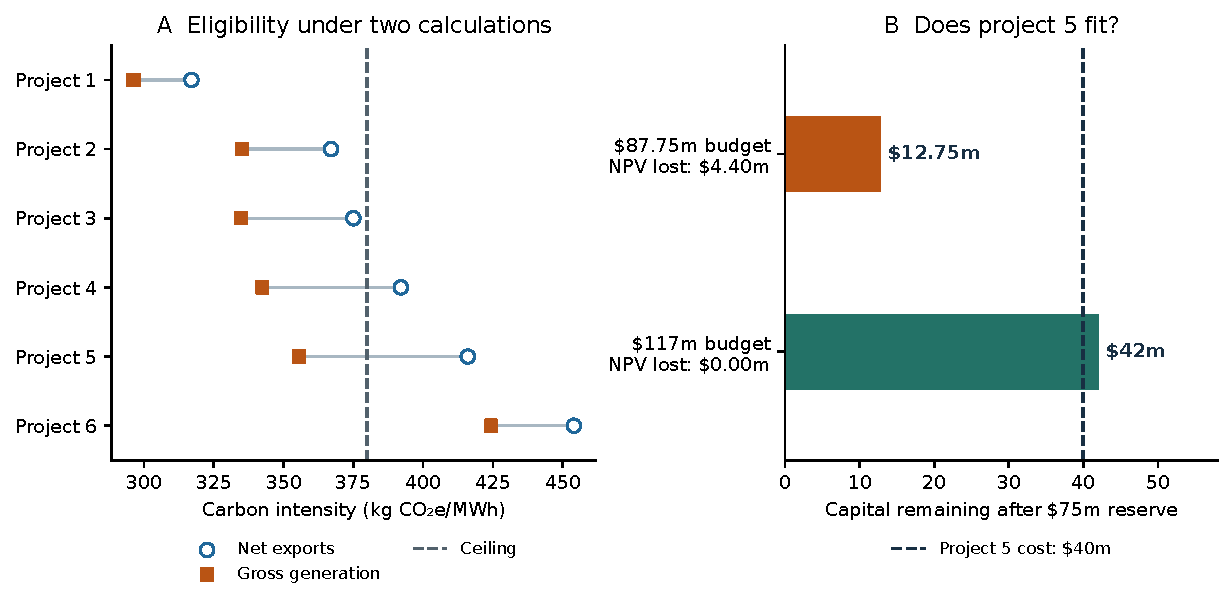
\includegraphics[width=\linewidth]{figures/project_example.pdf}
\caption{At one budget, admitting project~5 costs two other projects their funding. At the other, all three qualifying investments remain funded. (A) Each row shows a project in portfolio~1. Open circles use electricity exported to the grid and squares use all electricity generated. Scores at or below the dashed ceiling of 380~\unit\ qualify. (B) Reserving USD 75 million for projects~1--3 leaves the amounts shown by the bars. The dashed line marks project~5's USD 40 million cost. The losses are the net present value (NPV) of qualifying projects displaced.}\label{fig:project}

\end{figure*}
\fi



\subsection{What changes when projects cross the emissions ceiling?}
Across the 72 combinations of portfolio, budget and ceiling, the projects funded under the reference rule delivered a mean NPV of USD 14.97 million. Both errors that lowered measured intensity raised total portfolio NPV on average while reducing the NPV earned by qualifying projects (Table~\ref{tab:money}). The two errors changed 129 selections. In 55 of them the lender could add an ineligible project and keep its entire reference portfolio. These cases account for 31 changes under gross-output substitution and 24 under Scope~2 omission. In the other changed selections, the newly funded projects used capital needed by qualifying investments.
\ifdefined\readingcopy\ifdefined\readingcopy\begin{table*}[!t]\else\begin{table}[!ht]\fi\centering
\caption{How each carbon calculation changes funding relative to the specified formula. Each row covers 72 combinations of portfolio, ceiling and budget. The first two columns count decisions. The monetary columns report means in modeled USD millions. Qualified NPV includes only funded projects meeting the stated rule. Total NPV includes every funded project.}\label{tab:money}
\footnotesize\setlength{\tabcolsep}{4pt}
\begin{tabularx}{\linewidth}{@{}Xrrrrr@{}}\toprule
 & \shortstack[r]{Funded set\\changed} & \shortstack[r]{Positive\\shortfall} & \shortstack[r]{Ineligible\\capital} & \shortstack[r]{Qualified NPV\\shortfall} & \shortstack[r]{Change in\\total NPV}\\\midrule
Gross output & 63 & 32 & 48.833 & 1.974 & $+10.794$\\
Scope 2 omitted & 66 & 42 & 58.944 & 2.614 & $+13.316$\\
Net output understated & 69 & 69 & 0.000 & 13.237 & $-13.237$\\
Reference & 0 & 0 & 0.000 & 0.000 & 0.000\\\bottomrule
\end{tabularx}
\ifdefined\readingcopy\end{table*}\else\end{table}\fi
\fi



An error in the other direction removed projects from consideration entirely. Understating net exports raised measured intensity and wrongly excluded 57 of the 73 project--ceiling comparisons that qualified under the correct rule. All 69 resulting changes in funding reduced qualified NPV through exclusion. In the opposite direction, using gross generation wrongly admitted 44 of the 71 comparisons above the ceiling, and omitting Scope~2 admitted 53. Taken together, the 73 qualifying and 71 nonqualifying comparisons account for the 144 eligibility tests under each formula.

Eligibility alone did not determine whether funding changed. At least one project crossed the ceiling in 69 of the 72 financing decisions under gross substitution and in all 72 under each of the other errors. Allowing different formulas for different projects gave 1,848 combinations of eligibility patterns and financing decisions. Of these, 1,068 contained errors in both directions. Only 161 lost qualified value through both exclusion and ineligible spending (Equation~\eqref{eq:decompose}). A count of misclassified projects would miss that distinction.


\subsection{Which budgets and emissions ceilings change the funding decision?}
The original budget and ceiling settings lie in a particularly sensitive part of the policy range (Figure~\ref{fig:map}). Within the rectangle spanned by those settings, gross substitution changed the funded set over 92.4\% of the area on average across the eight portfolios. The corresponding shares were 98.3\% for Scope~2 omission and 97.8\% for net-output undercount. Across the full range of project scores and capital budgets, the three mean shares fell to 36.7\%, 42.8\% and 53.3\%. That range includes budgets too small to finance a project and ceilings at which the screens agree. Extending it beyond the lowest and highest calculated scores would add only unchanged allocations.
\ifdefined\readingcopy\begin{figure*}[!t]
\centering
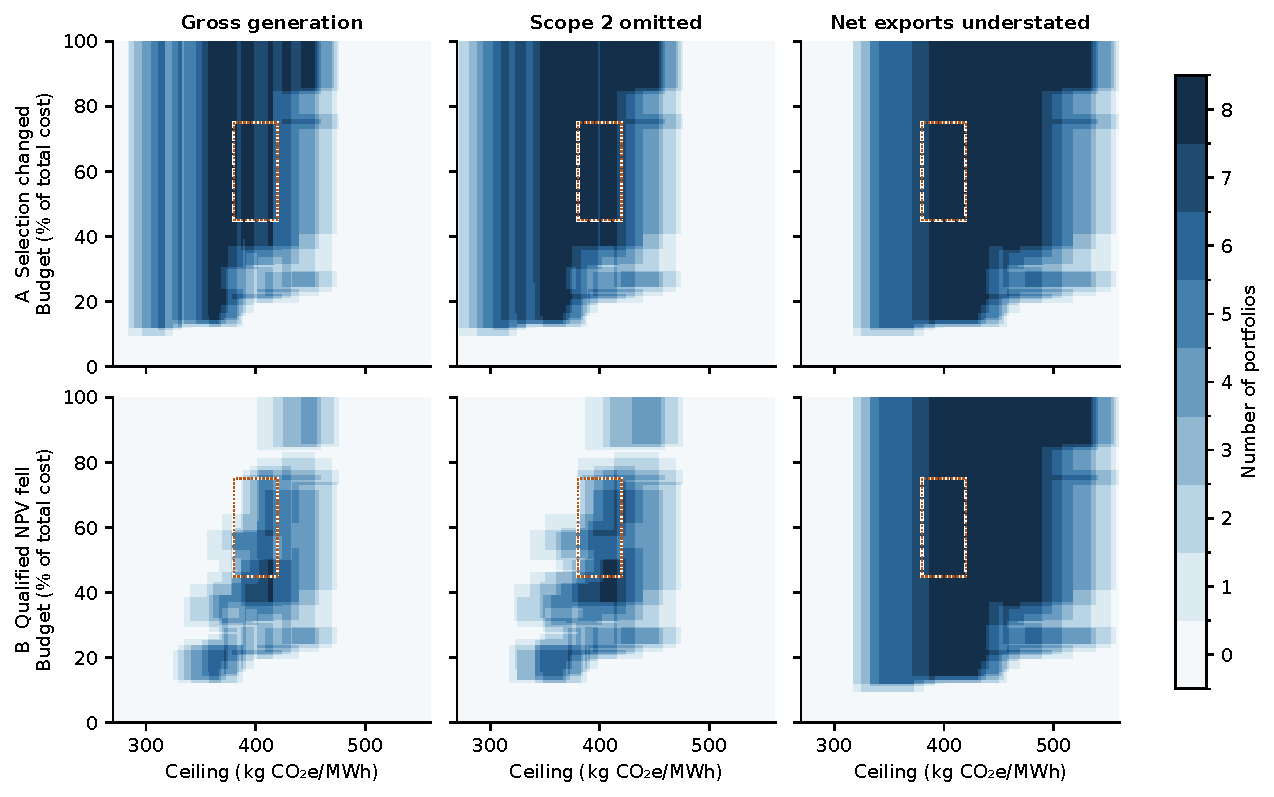
\includegraphics[width=\linewidth]{figures/policy_geometry.pdf}
\caption{Where a carbon calculation changes funding and where it reduces qualifying value. Each point represents an emissions ceiling and a budget. Within each column, the upper map (A) counts portfolios whose funded projects changed under the indicated error, and the lower map (B) counts those whose funded projects delivered less net present value under the stated eligibility rule. Both rows use the same scale from zero to eight portfolios. Boxes mark the original study range of 380--420~\unit\ and budgets of 45--75\% of the capital required for all six projects.}\label{fig:map}

\end{figure*}
\fi



Qualified NPV fell over a smaller share of the full rectangle under the two downward errors, averaging 12.1\% for gross substitution and 14.6\% for Scope~2 omission. Under net-output undercount, every change in selection reduced qualified NPV, giving 53.3\% for both outcomes.

A larger budget can finance more ineligible capital while displacing less qualified value. Between the original 45\% and 75\% budgets, gross substitution raised mean ineligible capital from USD 40.21 million to USD 54.13 million, while mean displacement fell from USD 3.51 million to USD 0.56 million. Extra capital could not restore projects excluded under net-output undercount. Its mean shortfall rose from USD 12.72 million to USD 13.62 million.

When the control projects started far from the ceiling, every one retained its eligibility. The smallest margin $|E_i-\tau|-|\widehat E_i-E_i|$ across the three altered formulas was 29.55~\unit, so every error fell short of the distance to the ceiling. All 216 decisions under the altered formulas retained the same funded sets as their 72 corresponding reference decisions.

\subsection{Comparing upward and downward errors of equal size}
On the original projects, overstating intensity cost more qualified NPV on average than understating it by a matched factor (Table~\ref{tab:matched}). For each of the three changes implemented in the code, we also calculated what would happen if the error acted in the opposite direction by the same factor. We used the exact ratios to settle cases that fell on the ceiling. With the fixed multiplier, the two directions changed the funded set equally often. Raising measured intensity nevertheless cost almost five times as much qualified NPV on average.
\ifdefined\readingcopy\ifdefined\readingcopy\begin{table*}[!t]\else\begin{table}[!ht]\fi\centering
\caption{Effects of lowering and raising intensity by the same factor. Each direction uses 72 portfolio, ceiling and budget combinations. Changes count funded sets that differ from the reference. Shortfalls are mean losses in qualified NPV, in modeled USD millions.}\label{tab:matched}
\footnotesize\begin{tabularx}{.98\linewidth}{@{}Xrrrr@{}}\toprule
 & \multicolumn{2}{c}{Lower intensity $E_i/m_i$} & \multicolumn{2}{c}{Higher intensity $E_i m_i$}\\
\cmidrule(lr){2-3}\cmidrule(l){4-5}
Factor $m_i$ & Changes & Shortfall & Changes & Shortfall\\\midrule
Gross/net output $G_i/Q_i$ &63&1.974&66&11.506\\
Inverse Scope 1 share $1/(1-s_i)$ &66&2.614&66&12.685\\
Inverse output multiplier $1/0.85$ &69&2.720&69&13.237\\\bottomrule
\end{tabularx}
\ifdefined\readingcopy\end{table*}\else\end{table}\fi
\fi



Changing which costs and cash flows belong to which project can reverse the ranking for an individual funding decision (Table~\ref{tab:assignment}). Each scale yielded 51,840 comparisons of the two directions at a given portfolio, pairing, ceiling and budget. Under one reassignment in portfolio~5, with a ceiling of 420 and a 45\% budget, using gross generation in place of net exports directed USD 79 million to projects above the ceiling. It displaced the entire USD 12.11 million in reference qualified NPV. The matched upward error lost only USD 0.60 million in qualified NPV.
\ifdefined\readingcopy\ifdefined\readingcopy\begin{table*}[!t]\else\begin{table}[!ht]\fi\centering
\caption{Difference in qualified NPV loss between raising intensity and lowering it after financial profiles are reassigned. A local reversal is one portfolio, budget, ceiling and assignment in which the downward error costs more. The full-grid range gives the lowest and highest attainable mean difference over all eight portfolios and nine policy settings, in modeled USD millions. Positive values mean the upward error costs more. The last three columns hold the budget fixed and weight the ceilings equally. Endpoints are rounded to two decimals.}\label{tab:assignment}
\footnotesize\setlength{\tabcolsep}{4pt}
\begin{tabularx}{\linewidth}{@{}Xrrrrr@{}}\toprule
 &\shortstack[r]{Local reversals\\of 51,840} & \shortstack[r]{Full grid\\sharp range} &\multicolumn{3}{c}{Lowest mean at fixed budget}\\
\cmidrule(l){4-6}
Factor & & & 45\% & 60\% & 75\%\\\midrule
Gross/net output & 2,098 & [1.60, 18.90] & $-1.83$ & $1.54$ & $3.84$\\
Inverse Scope 1 share & 1,748 & [1.69, 21.03] & $-1.90$ & $1.63$ & $4.27$\\
Inverse output multiplier & 740 & [1.67, 21.77] & $-1.77$ & $1.67$ & $4.77$\\\bottomrule
\end{tabularx}
\ifdefined\readingcopy\end{table*}\else\end{table}\fi
\fi



A positive difference in Table~\ref{tab:assignment} means that overstating intensity cost more qualified NPV. For the gross-to-net output factor, the smallest average difference across the full grid was USD 1.60 million. Holding the budget at 45\% instead, one assignment made understating intensity cost USD 1.83 million more on average. All three scales showed the same distinction. With equal weight on eight portfolios, three ceilings and three budgets, overstatement cost more on average under every joint assignment. At the 45\% budget, a single joint assignment gave differences of USD $-1.28$, $-1.90$ and $-0.90$ million for the gross-to-net, inverse Scope~1 and fixed scales, respectively, averaging equally across ceilings. At the 60\% and 75\% budgets, the lower bound was positive for every scale.

\subsection{How many checks identify the funded projects?}
When all six projects used the same formula, checking whether one project qualified could settle the funding decision for another. In portfolio~1 at the 380 ceiling and 45\% budget, project~4 had negative NPV and could never win funding. Yet once project~2 qualified, checking project~4 distinguished the correct formula from the two that lowered measured intensity. A check on a project with no investment value could therefore reveal which other projects qualified.

At most two checks identified the funded set at each of the 72 settings with a shared formula. Moving from the strictest formula to the most permissive only added eligible projects. Checking a project whose status differed across the possible formulas could therefore rule out several possibilities at once.

When projects could use different formulas, the answer for project~4 told the reviewer nothing about project~5. The reviewer could nevertheless stop once two selections agreed. These were the best portfolio using only projects certain to qualify and the best using every project that might qualify. That same portfolio wins for every intermediate set. If the two selections differ, either remains possible, and another check is needed. This raised the worst-case requirement to five checks. Adding the separate worst-case counts for all 72 decisions, choosing each check after seeing the previous answer required 135 checks under a shared formula, compared with 155 for the best lists fixed in advance. With project-specific formulas, both strategies took 285 checks. Resolving every uncertain project's status would have taken 330.

\subsection{What the source files reveal about a calculation error}
Across all 192 main files, LEAP extracted the indicator name and declared formula, anchored the record at line~1, and retained the nearby code containing the return expression at line~10. The formula declaration was on line~4. A simple program reading the first matching annotation recovered the same file names, normalized indicator names, formulas and KPI anchor lines across the four templates.

Comparing the written and implemented operations identified all 144 deliberately altered files. Running the programs on the project inputs and comparing their outputs with the expected values identified the same 144. The additional cases in Supplement~S1 show where the two checks diverge. Reordering the two terms in the numerator triggered a structural mismatch while preserving the numerical value. A stale declaration and matching implementation passed the structural comparison while returning 36 instead of the policy-reference intensity of 40 on the constructed inputs. To assess the financial consequence, the reviewer must follow that answer into the funding decision.

\section{Discussion}
For an investment committee examining a disputed carbon calculation, the amount committed outside the mandate is only the first number to establish. The next is how much capital the committee needs to retain the best investments that pass both screens. If several combinations deliver the same qualified NPV, the least expensive leaves the most money available. Once ineligible spending exceeds that amount, an entire qualifying project can fall out of reach. The value displaced depends on which alternatives the remaining budget can fund (Equation~\eqref{eq:slack}).

An erroneous admission can also raise the portfolio's total NPV. The financier may select a project for its positive NPV even though it fails the carbon screen. Reporting the capital committed outside the mandate alongside the qualified NPV shortfall distinguishes the size of that commitment from the value of the opportunities forgone. If the calculation also rejects qualified projects, Equation~\eqref{eq:decompose} first values those exclusions at the full budget, then measures the displacement among projects still eligible under both calculations. This accounting applies to an investment mandate with a fixed ceiling. A financier that assigns a monetary value to environmental outcomes faces a different investment decision \citep{schoenmaker}.

The distinction between a change in selection and a loss in value helps connect our findings to the carbon portfolio literature. Where \citet{anquetin} compared investment choices under different emissions measures, we held the lender's rule fixed and followed an error through the budget. In 55 of the 129 changed selections under the two errors that lowered measured intensity, the lender funded the entire reference portfolio alongside the newly admitted projects. A count of changed selections alone would have missed that outcome.

The original test ceilings lay close to several projects' calculated intensities. A small change in the formula could therefore move several projects across a ceiling at once. Including ceilings where the formulas agreed and budgets too small to fund a project reduced the share of settings affected (Figure~\ref{fig:map}).

The budget helps explain how much a change costs. At the tightest budget, reassigning financial profiles could make understating intensity more costly than overstating it by the same factor. With equal weight on the eight portfolios and nine budget--ceiling settings, overstatement cost more on average under every joint assignment at all three scales.

\subsection{Implications for environmental investment governance}
The findings connect carbon-accounting governance with the execution of a defined investment strategy. Where \citet{ruan2026} identify the organizational arrangements that embed emissions accounting, the displacement condition in Equation~\eqref{eq:slack} makes one consequence of implementation failure calculable at the capital-approval stage. The appropriate unit of assurance is the decision supported by the calculation: its approved rule, actual implementation, competing project set and capital budget. This operationalizes a narrow part of the measurement-to-accountability relationship described by \citet{tian2026}.

For an investment committee, three quantities distinguish mandate compliance from its financial consequences: capital committed outside the rule, qualified value forgone through exclusion, and qualified value displaced through erroneous admission. The first identifies exposure to nonconforming investment; the latter two are the components of the qualified NPV shortfall in Equation~\eqref{eq:decompose}. When the committee has verified the candidate projects and their costs and values, it can compare the ineligible commitments against the capital remaining after reserving the least expensive highest-NPV portfolio of projects that pass both calculations. This reveals whether a positive-NPV project admitted in error displaces qualified value, even when the nominal portfolio NPV rises. The evidence in Table~\ref{tab:money} shows why both financial quantities are useful.

Verification can then be directed toward the unresolved eligibility decisions that change the funding outcome. Under a shared uncertain formula, checking one informative project can resolve other projects' eligibility; where implementations vary independently, additional project-level checks may be necessary. The resulting verification certificates concern the selected portfolio under the specified alternatives. A proposed governance process would document the approved emissions boundary and denominator, record the executable formula and its version, re-evaluate eligibility, and retain the before-and-after allocation and loss decomposition as the decision record. Such a record gives sustainability assurance a concrete connection to capital approval, complementing firm-level studies of audit quality and reported carbon intensity \citep{ibrahim2026}.

\subsection{Scope and limitations}
The threshold applies to any finite set of indivisible projects with one budget, positive additive costs, additive values, and the option to leave funds unspent. If one project changes another's cash flows, or a covenant restricts which projects can be financed together, the remaining capital alone may no longer determine displacement.

One design produced all 48 projects in the eight portfolios. Reassigning their costs and cash flows preserves the financial profiles and relationships among emissions inputs. The policy map describes these projects across different ceilings and budgets. Estimating the frequency of errors, typical losses or effects on actual emissions would require project and lending records.

A field estimate would require isolating the formula error. At Copiulemu, methane revisions changed both a spreadsheet column and the assumed flare efficiency \citep[pp.~9--11, 14]{sgs}. Measuring the column's contribution would require holding flare efficiency and the other inputs fixed.

Valuing the alternatives requires financing records. The Vasilikos appraisal reports an emissions estimate and gives no indication of a coding defect. The loan register records the amount signed \citep{eibscore,eibloan}. Applying our screen would require knowing which emissions the bank counted and whether it used net exports. Measuring displacement would also require the competing proposals, their costs and cash flows, the budget and eligibility under both calculations.

The verification model assumes a known list of possible formulas and accurate, equally costly answers. With a shared formula, checking an unfunded project can reveal which others qualify. With project-specific formulas, it settles only that project's status. Partial sharing or unequal costs could change which check is worth doing first. Estimating analyst time would require measuring the work each answer takes.

\section{Conclusions}
A lender investigating a carbon calculation error can use its own project list to estimate the opportunity cost. Among projects that pass both calculations, find the least expensive portfolio that achieves the highest NPV the full budget allows. The capital left over is how much the lender can commit to ineligible projects before it displaces qualifying value. To measure the displacement in dollars, compare the best NPV those same qualifying projects can deliver at the full budget and at the budget left after the ineligible commitments. If the error also excluded qualifying projects, value those lost opportunities separately at the full budget.

\section*{Supporting information and data availability}
Supplement S1 contains the constructed project registers, annotated source files, original implementation and control results, and reproducibility scripts. It includes decision-level comparisons, the exclusion and displacement components, matched-direction and reassignment sensitivity, the full policy map, verification-count calculations and source-inspection cases. The replication repository identifier is provided separately with the author information.

\begin{thebibliography}{}
\setlength{\itemsep}{5pt plus 1pt}
\bibitem[Anquetin et al.(2022)]{anquetin} Anquetin, T., Coqueret, G., Tavin, B., \& Welgryn, L. (2022). Scopes of carbon emissions and their impact on green portfolios. \emph{Economic Modelling, 115}, 105951. \url{https://doi.org/10.1016/j.econmod.2022.105951}
\bibitem[Berg et al.(2022)]{berg} Berg, F., Kölbel, J.~F., \& Rigobon, R. (2022). Aggregate confusion: The divergence of ESG ratings. \emph{Review of Finance, 26}(6), 1315--1344. \url{https://doi.org/10.1093/rof/rfac033}
\bibitem[de Adelhart Toorop et al.(2024)]{schoenmaker} de Adelhart Toorop, R., Schoenmaker, D., \& Schramade, W. (2024). Decision rules for corporate investment. \emph{International Journal of Financial Studies, 12}(1), 24. \url{https://doi.org/10.3390/ijfs12010024}
\bibitem[Dughmi et al.(2026)]{dughmi} Dughmi, S., Kalayci, Y.~H., \& Liu, X. (2026). Near-optimal sparsifiers for stochastic knapsack and assignment problems. \emph{17th Innovations in Theoretical Computer Science Conference}, LIPIcs 362, 51:1--51:22. \url{https://doi.org/10.4230/LIPIcs.ITCS.2026.51}
\bibitem[European Investment Bank(2020a)]{eibscore} European Investment Bank. (2020a). \emph{EFSI Operation Scoreboard: EAC Vasilikos CCGT Unit 6}. 16 December, p.~1. \href{https://www.eib.org/attachments/registers/137305639.pdf}{EIB operation scoreboard}.
\bibitem[European Investment Bank(2020b)]{eibloan} European Investment Bank. (2020b). \emph{EAC Vasilikos CCGT Unit 6}. Project 20190376, financing signature of 17 December 2020. \href{https://www.eib.org/en/projects/all/20190376}{EIB project register}.
\bibitem[European Investment Bank(2023)]{eibmid} European Investment Bank. (2023). \emph{Mid-Term Review of the EIB Energy Lending Policy}. Annex~A, p.~26. \href{https://www.eib.org/attachments/lucalli/20230012_mid-term_review_of_the_energy_lending_policy_en.pdf}{EIB mid-term review}.
\bibitem[He et al.(2019)]{he} He, Y., Liao, N., Bi, J., \& Guo, L. (2019). Investment decision-making optimization of energy efficiency retrofit measures in multiple buildings under financing budgetary restraint. \emph{Journal of Cleaner Production, 215}, 1078--1094. \url{https://doi.org/10.1016/j.jclepro.2019.01.119}
\bibitem[Hien et al.(2026)]{hien} Hien, H.~T., Cha, J., Han, S.~M., Pham, L., \& Luong, H.~T.~H. (2026). When does uncertainty calibration exhaust the risk budget? Mathematical feasibility analysis and a convergence-audited neural--EWMA comparison. \emph{International Journal of Financial Studies, 14}(11), 327. \href{https://www.mdpi.com/2227-7072/14/11/327}{doi:10.3390/ijfs14110327}.
\bibitem[Ibrahim et al.(2026)]{ibrahim2026} Ibrahim, M.~B., Tingbani, I., \& Bassyouny, H. (2026). The impact of sustainability audit quality on corporate climate change performance: The role of governance quality and greenwashing. \emph{Business Strategy and the Environment}, e71508. \url{https://doi.org/10.1002/bse.71508}
\bibitem[Joshipura et al.(2025)]{joshipura2025} Joshipura, M., Nasrallah, N., \& Kedia, N. (2025). Green and climate finance for sustainability: Hybrid review and framework development. \emph{Business Strategy and the Environment, 34}, 3618--3634. \url{https://doi.org/10.1002/bse.4173}
\bibitem[Knuth(1984)]{knuth} Knuth, D.~E. (1984). Literate programming. \emph{The Computer Journal, 27}(2), 97--111. \url{https://doi.org/10.1093/comjnl/27.2.97}
\bibitem[Lohmann et al.(2026)]{lohmann} Lohmann, C., Möllenhoff, S., \& Lehner, S. (2026). ESG rating disagreement and the size of the investable universe under ESG consensus rules. \emph{Corporate Social Responsibility and Environmental Management, 33}(2), 2649--2664. \url{https://doi.org/10.1002/csr.70313}
\bibitem[Loiola et al.(2026)]{loiola} Loiola, R.~R., de Melo Souza, L., \& Kimura, H. (2026). Green bond alignment, certification and corporate credit risk: Evidence from global issuers. \emph{International Journal of Financial Studies, 14}(9), 244. \url{https://doi.org/10.3390/ijfs14090244}
\bibitem[Lorie and Savage(1955)]{lorie} Lorie, J.~H., \& Savage, L.~J. (1955). Three problems in rationing capital. \emph{The Journal of Business, 28}(4), 229--239. \url{https://doi.org/10.1086/294081}
\bibitem[Mouawad(2026a)]{zenodo} Mouawad, M. (2026a). \emph{LEAP: Automating KPI Documentation in Enterprise Codebases through Literate Programming and AI}. Zenodo, version~1. \url{https://doi.org/10.5281/zenodo.20764919}
\bibitem[Mouawad(2026b)]{leap} Mouawad, M.~O. (2026b). \emph{Reconstructing Source-Linked KPI Documentation: Architecture and Evaluation of LEAP}. Research manuscript, version P6R17. \href{https://github.com/Meshaal-Mouawad/LEAP-Paper1-Evidence/blob/a20b243683a262fd43987013117120c313ec8fa8/SCP_P6R17/01_Manuscript_SCP_P6R17.pdf}{Author's archived manuscript}.
\bibitem[Mouawad(2026c)]{review} Mouawad, M. (2026c). A source-linked review method for KPI definition--implementation disagreements. \emph{Research Square}, preprint, version~1. \url{https://doi.org/10.21203/rs.3.rs-11525474/v1}
\bibitem[Mouawad and Jones(2026)]{checks} Mouawad, M.~O., \& Jones, B. (2026). \emph{Evaluating Checks for Generated KPI Documentation: Rule Coverage and Reference Criteria}. Manuscript under peer review at \emph{Science of Computer Programming} (SCICO-D-26-00865). \href{https://github.com/Meshaal-Mouawad/Paper_2_JSS/blob/1fe7d8c1efe0e90b036f81ae319fbcffb80a262a/main.pdf}{Author manuscript and replication materials}.
\bibitem[Nicolici et al.(2026)]{nicolici} Nicolici, V.-S., Adjal, A., Ionel, I., \& Grecu, E. (2026). Integrated management of air-quality monitoring processes as a framework for disclosure quality in green bond markets. \emph{International Journal of Financial Studies, 14}(7), 168. \url{https://doi.org/10.3390/ijfs14070168}
\bibitem[Pisinger and Saidi(2017)]{pisinger} Pisinger, D., \& Saidi, A. (2017). Tolerance analysis for 0--1 knapsack problems. \emph{European Journal of Operational Research, 258}(3), 866--876. \url{https://doi.org/10.1016/j.ejor.2016.10.054}
\bibitem[Raimondi et al.(2026)]{raimondi2026} Raimondi, R., Schwizer, P.~G.~M., Cosma, S., \& Rimo, G. (2026). Credit risk assessment in the climate shadow: Evidence from white and grey literature. \emph{Business Strategy and the Environment, 35}, 2526--2546. \url{https://doi.org/10.1002/bse.70276}
\bibitem[Ruan et al.(2026)]{ruan2026} Ruan, L., Sahore, N., Almasabi, S.~S., Di Vaio, A., \& Papa, A. (2026). A strategic governance perspective on carbon accounting enablers: An in-depth qualitative examination of business strategies. \emph{Business Strategy and the Environment}, e71537. \url{https://doi.org/10.1002/bse.71537}
\bibitem[Schl\"oter(2025)]{schloter} Schlöter, J. (2025). On the complexity of knapsack under explorable uncertainty: Hardness and algorithms. \emph{33rd Annual European Symposium on Algorithms}, LIPIcs 351, 6:1--6:15. \url{https://doi.org/10.4230/LIPIcs.ESA.2025.6}
\bibitem[SGS United Kingdom(2008)]{sgs} SGS United Kingdom Ltd. (2008). \emph{Verification and Certification Report: Copiulemu Landfill Gas Project}. CDM.Ver0036, UNFCCC project 0096, 30 July, pp.~10--11. \href{https://cdm.unfccc.int/Projects/DB/DNV-CUK1126875537.72/iProcess/SGS-UKL1188294574.74/ReviewInitialComments/NEXNYPXPNJFC9OOG8BF6DBO3EOC9Q4}{UNFCCC project archive}.
\bibitem[Tian(2026)]{tian2026} Tian, G.~G. (2026). ESG measurement and ratings divergence: A cross-jurisdictional review of institutional, stakeholder, and digital accountability perspectives. \emph{Business Strategy and the Environment}. Advance online publication. \url{https://doi.org/10.1002/bse.71005}
\bibitem[United Nations(n.d.)]{un} United Nations. (n.d.). \emph{Goal 7: Ensure Access to Affordable, Reliable, Sustainable and Modern Energy for All}. Target~7.a. Department of Economic and Social Affairs. \url{https://sdgs.un.org/goals/goal7}.
\bibitem[WRI and WBCSD(2004)]{ghg} World Resources Institute and World Business Council for Sustainable Development. (2004). \emph{The Greenhouse Gas Protocol: A Corporate Accounting and Reporting Standard}, revised edition. \href{https://ghgprotocol.org/sites/default/files/standards/ghg-protocol-revised.pdf}{Greenhouse Gas Protocol}.
\bibitem[Wu et al.(2026)]{wu2026} Wu, W., Alghafes, R., Sahore, N., Battisti, E., \& Liu, X. (2026). The nitty gritty of carbon accounting: Enablers, barriers, reporting, and strategies. \emph{Business Strategy and the Environment, 35}, 8380--8405. \url{https://doi.org/10.1002/bse.70490}
\end{thebibliography}

\ifdefined\readingcopy
\else
  \onecolumn
  \section*{Tables}
  \ifdefined\readingcopy\begin{table*}[!t]\else\begin{table}[!ht]\fi\centering
\caption{How each carbon calculation changes funding relative to the specified formula. Each row covers 72 combinations of portfolio, ceiling and budget. The first two columns count decisions. The monetary columns report means in modeled USD millions. Qualified NPV includes only funded projects meeting the stated rule. Total NPV includes every funded project.}\label{tab:money}
\footnotesize\setlength{\tabcolsep}{4pt}
\begin{tabularx}{\linewidth}{@{}Xrrrrr@{}}\toprule
 & \shortstack[r]{Funded set\\changed} & \shortstack[r]{Positive\\shortfall} & \shortstack[r]{Ineligible\\capital} & \shortstack[r]{Qualified NPV\\shortfall} & \shortstack[r]{Change in\\total NPV}\\\midrule
Gross output & 63 & 32 & 48.833 & 1.974 & $+10.794$\\
Scope 2 omitted & 66 & 42 & 58.944 & 2.614 & $+13.316$\\
Net output understated & 69 & 69 & 0.000 & 13.237 & $-13.237$\\
Reference & 0 & 0 & 0.000 & 0.000 & 0.000\\\bottomrule
\end{tabularx}
\ifdefined\readingcopy\end{table*}\else\end{table}\fi

  \ifdefined\readingcopy\begin{table*}[!t]\else\begin{table}[!ht]\fi\centering
\caption{Effects of lowering and raising intensity by the same factor. Each direction uses 72 portfolio, ceiling and budget combinations. Changes count funded sets that differ from the reference. Shortfalls are mean losses in qualified NPV, in modeled USD millions.}\label{tab:matched}
\footnotesize\begin{tabularx}{.98\linewidth}{@{}Xrrrr@{}}\toprule
 & \multicolumn{2}{c}{Lower intensity $E_i/m_i$} & \multicolumn{2}{c}{Higher intensity $E_i m_i$}\\
\cmidrule(lr){2-3}\cmidrule(l){4-5}
Factor $m_i$ & Changes & Shortfall & Changes & Shortfall\\\midrule
Gross/net output $G_i/Q_i$ &63&1.974&66&11.506\\
Inverse Scope 1 share $1/(1-s_i)$ &66&2.614&66&12.685\\
Inverse output multiplier $1/0.85$ &69&2.720&69&13.237\\\bottomrule
\end{tabularx}
\ifdefined\readingcopy\end{table*}\else\end{table}\fi

  \ifdefined\readingcopy\begin{table*}[!t]\else\begin{table}[!ht]\fi\centering
\caption{Difference in qualified NPV loss between raising intensity and lowering it after financial profiles are reassigned. A local reversal is one portfolio, budget, ceiling and assignment in which the downward error costs more. The full-grid range gives the lowest and highest attainable mean difference over all eight portfolios and nine policy settings, in modeled USD millions. Positive values mean the upward error costs more. The last three columns hold the budget fixed and weight the ceilings equally. Endpoints are rounded to two decimals.}\label{tab:assignment}
\footnotesize\setlength{\tabcolsep}{4pt}
\begin{tabularx}{\linewidth}{@{}Xrrrrr@{}}\toprule
 &\shortstack[r]{Local reversals\\of 51,840} & \shortstack[r]{Full grid\\sharp range} &\multicolumn{3}{c}{Lowest mean at fixed budget}\\
\cmidrule(l){4-6}
Factor & & & 45\% & 60\% & 75\%\\\midrule
Gross/net output & 2,098 & [1.60, 18.90] & $-1.83$ & $1.54$ & $3.84$\\
Inverse Scope 1 share & 1,748 & [1.69, 21.03] & $-1.90$ & $1.63$ & $4.27$\\
Inverse output multiplier & 740 & [1.67, 21.77] & $-1.77$ & $1.67$ & $4.77$\\\bottomrule
\end{tabularx}
\ifdefined\readingcopy\end{table*}\else\end{table}\fi

  \clearpage
  \section*{Figure legends}
\begin{figure}[!ht]
\centering

\caption{At one budget, admitting project~5 costs two other projects their funding. At the other, all three qualifying investments remain funded. (A) Each row shows a project in portfolio~1. Open circles use electricity exported to the grid and squares use all electricity generated. Scores at or below the dashed ceiling of 380~\unit\ qualify. (B) Reserving USD 75 million for projects~1--3 leaves the amounts shown by the bars. The dashed line marks project~5's USD 40 million cost. The losses are the net present value (NPV) of qualifying projects displaced.}\label{fig:project}

\end{figure}
\begin{figure}[!ht]
\centering

\caption{Where a carbon calculation changes funding and where it reduces qualifying value. Each point represents an emissions ceiling and a budget. Within each column, the upper map (A) counts portfolios whose funded projects changed under the indicated error, and the lower map (B) counts those whose funded projects delivered less net present value under the stated eligibility rule. Both rows use the same scale from zero to eight portfolios. Boxes mark the original study range of 380--420~\unit\ and budgets of 45--75\% of the capital required for all six projects.}\label{fig:map}

\end{figure}
\clearpage
\fi
\end{document}
